\documentclass[10pt,leter,openany]{article}
\usepackage[latin1]{inputenc}
\usepackage[english]{babel}
\usepackage{amsmath}
\usepackage{amsfonts}
\usepackage{amssymb}
\usepackage{graphicx}
\usepackage{listings}
\usepackage{color}
\usepackage[left=3cm,right=3cm,top=3cm,bottom=3cm]{geometry}
\usepackage[numbers,sort&compress]{natbib}
\usepackage{url}
\usepackage{caption}
\usepackage{siunitx}
%\usepackage{subfigure}
\usepackage{float}
\usepackage{booktabs}
\usepackage{subcaption}
\usepackage{comment}
\usepackage{mwe}
%\usepackage[table,xcdraw]{xcolor}

\setlength{\parindent}{0pt}
\setlength{\parskip}{4pt}

\definecolor{mygreen}{rgb}{0,0.6,0}
\definecolor{mygray}{rgb}{0.5,0.5,0.5}
\definecolor{mymauve}{rgb}{0.58,0,0.82}

\lstset{ 
	backgroundcolor=\color{white},   % choose the background color; you must add \usepackage{color} or \usepackage{xcolor}; should come as last argument
	basicstyle=\footnotesize,        % the size of the fonts that are used for the code
	breakatwhitespace=false,         % sets if automatic breaks should only happen at whitespace
	breaklines=true,                 % sets automatic line breaking
	captionpos=b,                    % sets the caption-position to bottom
	commentstyle=\color{mygreen},    % comment style
	deletekeywords={...},            % if you want to delete keywords from the given language
	escapeinside={\%*}{*)},          % if you want to add LaTeX within your code
	extendedchars=true,              % lets you use non-ASCII characters; for 8-bits encodings only, does not work with UTF-8
	firstnumber=01,                	 % start line enumeration with line 1000
	frame=single,	                 % adds a frame around the code
	keepspaces=true,                 % keeps spaces in text, useful for keeping indentation of code (possibly needs columns=flexible)
	keywordstyle=\color{blue},       % keyword style
	language=Python,                 % the language of the code
	morekeywords={*,...},            % if you want to add more keywords to the set
	numbers=left,                    % where to put the line-numbers; possible values are (none, left, right)
	numbersep=5pt,                   % how far the line-numbers are from the code
	numberstyle=\tiny\color{mygray}, % the style that is used for the line-numbers
	rulecolor=\color{black},         % if not set, the frame-color may be changed on line-breaks within not-black text (e.g. comments (green here))
	showspaces=false,                % show spaces everywhere adding particular underscores; it overrides 'showstringspaces'
	showstringspaces=false,          % underline spaces within strings only
	showtabs=false,                  % show tabs within strings adding particular underscores
	stepnumber=1,                    % the step between two line-numbers. If it's 1, each line will be numbered
	stringstyle=\color{mymauve},     % string literal style
	tabsize=2,	                     % sets default tabsize to 2 spaces
	title=\lstname                   % show the filename of files included with \lstinputlisting; also try caption instead of title
}

\usepackage[dvipsnames,table,xcdraw]{xcolor}

\usepackage{fancyvrb}

% redefine \VerbatimInput
\RecustomVerbatimCommand{\VerbatimInput}{VerbatimInput}%
{fontsize=\footnotesize,
	%
	frame=lines,  % top and bottom rule only
	framesep=2em, % separation between frame and text
	rulecolor=\color{Gray},
	%
	label=\fbox{\color{Black}data.txt},
	labelposition=topline,
	%
	commandchars=\|\(\), % escape character and argument delimiters for
	% commands within the verbatim
	commentchar=*        % comment character
}



\usepackage{titling}
\newcommand{\subtitle}[1]{%
	\posttitle{%
		\par\end{center}
	\begin{center}\large#1\end{center}
	\vskip0.5em}%
}


\author{5273}
\title{Homework Assignment 6: Applied Probabilistic Models}
\subtitle{Statistical Tests}
\date{}


\begin{document}
	
\maketitle

\section{Introduction}
	
	For this work, data is collected on the official website of Instituto Nacional de Estad�stica y Geograf�a (INEGI) \citep{inegi_data}. The chosen section is Growth Domestic Product, and within this section, a national macroeconomic indicator is selected: Global Index of Economic Activity (IGAE) for the data analysis. Data obtained from INEGI website are in \texttt{csv} format, edited in order to work with the general values of the three main representative activities each month, which the aforementioned indicator is based on.
	
	For the analysis it is used the R software in its version 4.0.2 \citep{r} and the code used is available on the GitHub repository of  \citep{github}. This work is run on a MacBook Air with an Intel Core i5 CPU $ @ $ 1.8 GHz and 8 GB RAM.
	
\section{Theoretical Aspects}
	
	This section covers several aspects of statistical and tests and when it is appropriate to use them and their interpretation. Characteristics of hypothesis tests are treated as well.
	
	\subsection{Hypothesis and statistical tests}
	
		A statistical test is a form of evaluating the evidence that data provide. The objective is to prove a hypothesis which is denominated as the null hypothesis ($H_{0}$). Typically, $H_{0}$ establishes equality (between means, variances, or correlation coefficient to cite some examples). $H_{0}$ usually opposed to a hypothesis denominate alternative ($H_{1}$) and implies difference (between means, for example).
	
	\subsection{Rejecting the null hypothesis}
	
		If data do not provide sufficient evidence against $H_{0}$, it is not rejected. If, contrary, show strong evidence against $H_{0}$ it is rejected, and $H_{1}$ it is considered as true with a quantified risk (low) of being wrong.
	
	\subsection{Interpretation of a statistical test}
	
		The statistical test produces a number denominated $p$-value, which limits are 0 and 1. The $p$-value is the probability of obtaining data or extreme data below the null hypothesis.
	
		In more pr�ctical terms, $p$-value should be compared with alpha (see subsection \ref{alpha_subsection}) and it can be interpreted follow:
		\begin{itemize}
			\item If $p < $ alpha, $H_{0}$ is rejected, and $H_{1}$ is  accepted with a proportional risk of the $p$-value of being wrong.
			\item If $p > $ alpha, $H_{0}$ is not rejected, but this does not imply it is necessary to be accepted. It means $H_{0}$ is true, but the experiment and the statistical test are not ``strong" enough to produce a $p$-value less than alpha.
		\end{itemize} 
	\subsection{Selecting alpha}\label{alpha_subsection}
	
		When a study is designed, a risk threshold must be specified, above which $H_{0}$ should not be rejected. This threshold is known as significance level, also denoted as alpha or $\alpha $, and should be between 0 and 1. Low alpha values are more conservative \citep{xlstat}.
	
		The selection of alpha should depend on how dangerous is reject $H_{0}$ in case it is true. For example, in a study to prove the benefits of medical treatment, alpha should be low. On the other hand, when revising effects of many attributes in the appreciation of a product, alpha could be moderate. In most cases, alpha is set at 0.05, 0.01, or 0.001.
	
	\subsection{Common mistakes when interpreting $p$-value}
	
		A mistake that can be made when interpreting p-value is if a study is realized two times and $p \leq 0.05$ in one case and $p > 0.05$ in another, its results are in conflict. This is a mistake to assume because most of the experimental series should throw some null result. Another one is when $p \leq 0.05$  assures that 95\% of effects will be true. The true probability that a significative effect reflects the existence of a real effect is given by the Positive Predictive Value (PPV), and it depends on the statistical power, plausibility of alternative hypotheses, and other questionable research practices. Another one is that a $p > 0.05$ implies there is no effect. This may be, but the truth is that there is no power enough to detect it. The other one is that $p \leq 0.05$ implies a found effect. The valid use of $p$-value is to control the rate of error type 1. The$p$-value does not say anything about concrete cases (current experiment) it only provides a general rule of behaviour \citep{perales2018}.
		
	\subsection{Statistical power}
	
		When various statistical tests are available to be used, it is critical to choose the most convenient and powerful for the experimental design to be used. For that reason, it is necessary a  selection criterion \citep{ecured}. One of them is the statistical power which is the probability of rejecting the null hypothesis when it is false. Therefore, it can be considered a statistical test as appropriate when the probability of rejecting the null hypothesis ($H_{0}$) is small when is true; and big enough the probability of rejecting it when is false.
	
	\subsection{Parametric and non-parametric statistical tests}
	
		Parametric tests are for numerical data and, in general, are based on the normal or gaussian distribution. Possible tests to apply are $t$-student, the Pearson correlation coefficient, linear regression, one-way Analysis of variance (One-way ANOVA), factorial analysis of variance (ANOVA), and Analysis of covariance (ANCOVA). Descriptive statistics such as standard deviation, mode, median and mean are used.
	
		On the other hand, non-parametric tests are used with nominal and ordinal variables. They do not assume a particular distribution and the requirements regarding sample size are not as many as the parametric ones. Most used tests are Chi-Squared, Correlation and independency coefficients for cross-tabulation and Spearman's and Kendall's rank correlation coefficient.
	
	\subsection{Guide to find the needed statistical test}
	
		To begin with, the objective of the analysis needs to be clear.  It could be about association or comparison. Both seek to establish relations (similarities or differences) between elements, but tests of comparison, in contrast with a test of association, evaluate relations between one or various groups. The type of variables has to be noticed (numeric or nominal) as well. Then, it needs to be distinguished if samples are independent or related. The next step corresponds to the fulfilment of the classical assumptions (Normality, homogeneity of variance, independency), this allows to choose between parametric, non-parametric and robust tests. Then, it can be chosen the appropriate test with the help of Table \ref{tab:map}. Once the test is selected, the next step is to perform hypothesis testing, and finally it corresponds to the interpretation and if possible graph the results.

		\begin{table}[]
			\centering
			\caption{Map to select the appropriate test}
			\label{tab:map}
			\resizebox{\textwidth}{!}{%
				\begin{tabular}{|lcl|l|l|l|}
					\hline
					\rowcolor[HTML]{FFFFFF} 
					&                                                                                                                                          & \multicolumn{4}{c|}{\cellcolor[HTML]{FFFFFF}\textit{\textbf{Data type}}}                                                                                                                                                                                                                                                                                                                                                                                                                              \\ \cline{2-6} 
					\rowcolor[HTML]{FFFFFF} 
					\multicolumn{1}{|c|}{\cellcolor[HTML]{FFFFFF}\textbf{}}                   & \multicolumn{1}{l|}{\cellcolor[HTML]{FFFFFF}}                                                                                            & \multicolumn{1}{c|}{\cellcolor[HTML]{FFFFFF}\textbf{\begin{tabular}[c]{@{}c@{}}Numeric \\ (gaussian)\end{tabular}}} & \multicolumn{1}{c|}{\cellcolor[HTML]{FFFFFF}\textbf{\begin{tabular}[c]{@{}c@{}}Ordinal or \\ numeric \\ (non gaussian)\end{tabular}}} & \multicolumn{1}{c|}{\cellcolor[HTML]{FFFFFF}\textbf{\begin{tabular}[c]{@{}c@{}}Numeric \\ (outliers)\end{tabular}}} & \multicolumn{1}{c|}{\cellcolor[HTML]{FFFFFF}\textbf{\begin{tabular}[c]{@{}c@{}}Nominal \\ (binary)\end{tabular}}} \\ \cline{2-6} 
					\rowcolor[HTML]{EFEFEF} 
					\multicolumn{1}{|l|}{\cellcolor[HTML]{FFFFFF}\textbf{}}                   & \multicolumn{1}{c|}{\cellcolor[HTML]{EFEFEF}\textbf{\begin{tabular}[c]{@{}c@{}}Compare 2 \\ independent \\ groups\end{tabular}}}         & \begin{tabular}[c]{@{}l@{}}$t$-student test \\ for 2 independent\\ samples\end{tabular}                             & \begin{tabular}[c]{@{}l@{}}Mann-Whitney\\ Test\end{tabular}                                                                           & \begin{tabular}[c]{@{}l@{}}Yuen test for\\ independent\\ samples\end{tabular}                                       & \begin{tabular}[c]{@{}l@{}}Fisher or \\ Chi-Squared\\ (for bigger samples)\end{tabular}                           \\
					\rowcolor[HTML]{FFFFFF} 
					\multicolumn{1}{|l|}{\cellcolor[HTML]{FFFFFF}}                            & \multicolumn{1}{c|}{\cellcolor[HTML]{FFFFFF}\textbf{\begin{tabular}[c]{@{}c@{}}Compare 2 \\ related groups\end{tabular}}}                & \begin{tabular}[c]{@{}l@{}}$t$-student test for 2\\ related samples\end{tabular}                                    & \begin{tabular}[c]{@{}l@{}}Wilcoxon Test\\ for related\\ samples\end{tabular}                                                         & \begin{tabular}[c]{@{}l@{}}Yuen Test for \\ related samples\end{tabular}                                            & McNemar Test                                                                                                      \\
					\rowcolor[HTML]{EFEFEF} 
					\multicolumn{1}{|l|}{\cellcolor[HTML]{FFFFFF}\textit{\textbf{Objective}}} & \multicolumn{1}{c|}{\cellcolor[HTML]{EFEFEF}\textbf{\begin{tabular}[c]{@{}c@{}}Compare 3 or \\ more independent \\ groups\end{tabular}}} & \begin{tabular}[c]{@{}l@{}}ANOVA one-way\\ for independent\\ samples\end{tabular}                                   & \begin{tabular}[c]{@{}l@{}}Kruskall-Wallis\\ Test\end{tabular}                                                                        & \begin{tabular}[c]{@{}l@{}}Robust ANOVA\\ one-way for\\ independent smples\end{tabular}                             & Chi-Squared Test                                                                                                  \\
					\rowcolor[HTML]{FFFFFF} 
					\multicolumn{1}{|l|}{\cellcolor[HTML]{FFFFFF}}                            & \multicolumn{1}{c|}{\cellcolor[HTML]{FFFFFF}\textbf{\begin{tabular}[c]{@{}c@{}}Compare 3 or \\ more related \\ groups\end{tabular}}}     & \begin{tabular}[c]{@{}l@{}}ANOVA one-way \\ for related samples\end{tabular}                                        & Friedman Test                                                                                                                         & \begin{tabular}[c]{@{}l@{}}Robust ANOVA \\ one-way \\ for related samples\end{tabular}                              & \begin{tabular}[c]{@{}l@{}}$Q$ of Cochrane\\ Test\end{tabular}                                                    \\
					\rowcolor[HTML]{EFEFEF} 
					\multicolumn{1}{|l|}{\cellcolor[HTML]{FFFFFF}}                            & \multicolumn{1}{c|}{\cellcolor[HTML]{EFEFEF}\textbf{\begin{tabular}[c]{@{}c@{}}Associate 2\\ variables\end{tabular}}}                    & \begin{tabular}[c]{@{}l@{}}Pearson \\ correlation\end{tabular}                                                      & \begin{tabular}[c]{@{}l@{}}Spearman\\ or Kendall \\ correlation\end{tabular}                                                          & \begin{tabular}[c]{@{}l@{}}Robust \\ correlation\end{tabular}                                                       & \begin{tabular}[c]{@{}l@{}}Cramer \\ $V$ coefficient\end{tabular}                                                 \\ \hline
				\end{tabular}%
			}
		\end{table}
	
	\subsection{Assumptions to apply parametric techniques}
	
		To apply parametric techniques the following assumptions are needed:
		\begin{itemize}
			\item Observations are independent of each other.
			\item Populations should be normally distributed.
			\item These populations must have the same variance.
			\item Variables must be measured on at least an interval scale so that arithmetic operations can be used.
		\end{itemize}
	
\section{Application of Statistical Tests}

 	In this section, several of the most used statistical tests are performed. These tests are applied considering data of the IGAE obtained from the INEGI website. The IGAE  is an index that approximates the calculation of the generated wealth in the country monthly. It is considered a trend index and marks the path that the national economic activity is reporting in the given month \citep{mvs}. The method used to calculate the IGAE consists of monthly indexes of the physical volume of production for each of the selected classes, with a fixed base in 2013 \citep{calculo_igae}. In the calculation of the IGAE, three fundamental areas or activities are involved: primary, secondary, and tertiary which are the ones analyzed in this work.

	\subsection{One Sample $t$-Test}
	
		This parametric test is used to test if the mean of a sample from a normal distribution could reasonably be a specific value \citep{selva2016}. In this case, data belong to the primary activities. The $p$-value is 0.4594, so the null hypothesis that the mean=90 cannot be rejected.
		
		\VerbatimInput{extras/t_test.txt}
		
		
		\subsection{Wilcoxon Signed Rank Test}
		
		This test can be considered as an alternative to $ t $-Test, especially when the data sample is not assumed to follow a normal distribution and it is a non-parametric method \citep{selva2016}. For this test, data belong to secondary activities. The $p$-value is less than the significance level of 0.05, so the null hypothesis is rejected and accept the alternative that true mean is not equal to 90.
		
		\VerbatimInput{extras/wilcoxon.txt}
		
		\subsection{Two Sample t-Test and Wilcoxon Rank Sum Test}
		
		Here both $ t $-Test and Wilcoxon rank test are used to compare the mean of 2 samples, passing the numeric vectors of primary and secondary activities. The $p$-value is 0.9976, so the null hypothesis cannot be rejected.
		
		\VerbatimInput{extras/wilcoxon_2sample.txt}

		\subsection{Shapiro Test}
		
		This is used to test if a sample follows a normal distribution. Data belong to primary activities. In this case, $p$-value is $3.29 \times 10^{-10}$, so the null hypothesis is rejected, which means data are not normally distributed. Figure \ref{fig:hist} shows a histogram of the values reached by primary activities.
		
		\begin{figure}
			\begin{center}
				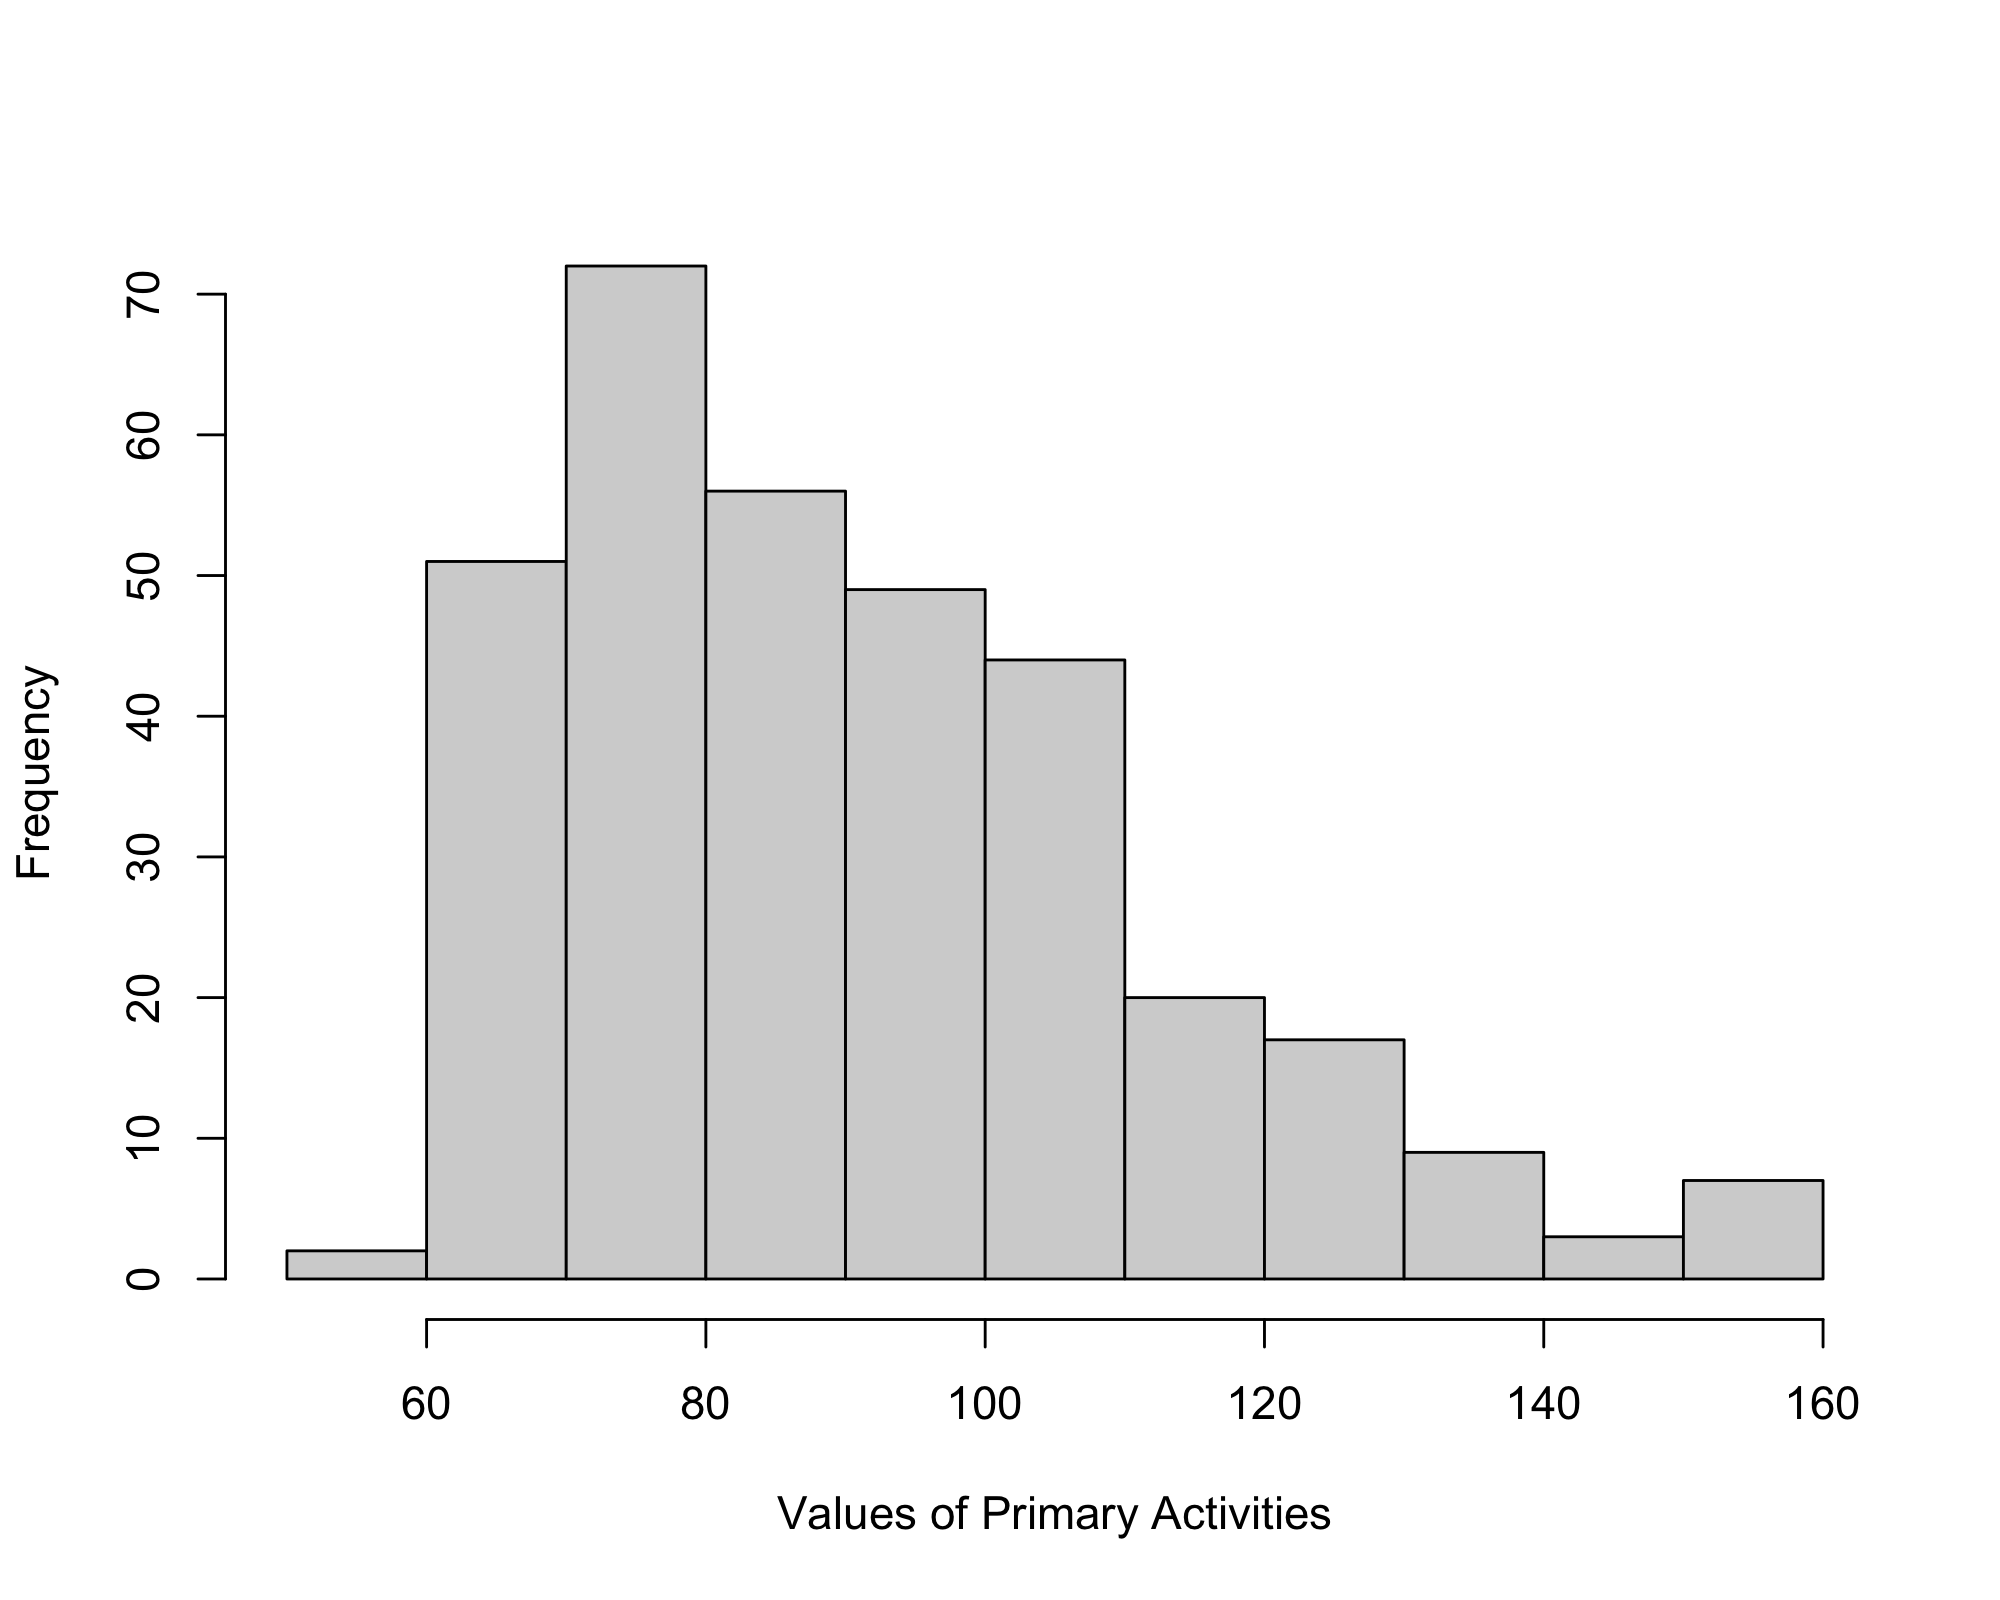
\includegraphics[scale=0.15]{extras/hist}
				\captionof{figure}{Histogram of the values of Primary Activiites}
				\label{fig:hist}
			\end{center}
		\end{figure}
		
		\VerbatimInput{extras/shapiro.txt}
		
		\subsection{Kolmogorov-Smirnov Test}
		
		This test is used to check whether two samples follow the same distribution. In this case, data belong to primary and secondary activities; the $p$-value is $3.70\times 10^{-10}$, so the null hypothesis is rejected, which means data do not come from the same distribution. A violin plot is generated in Figure \ref{fig:violin} to show how both groups are distributed.
		
		
		\VerbatimInput{extras/ks.txt}
		
		\begin{figure}
			\begin{center}
				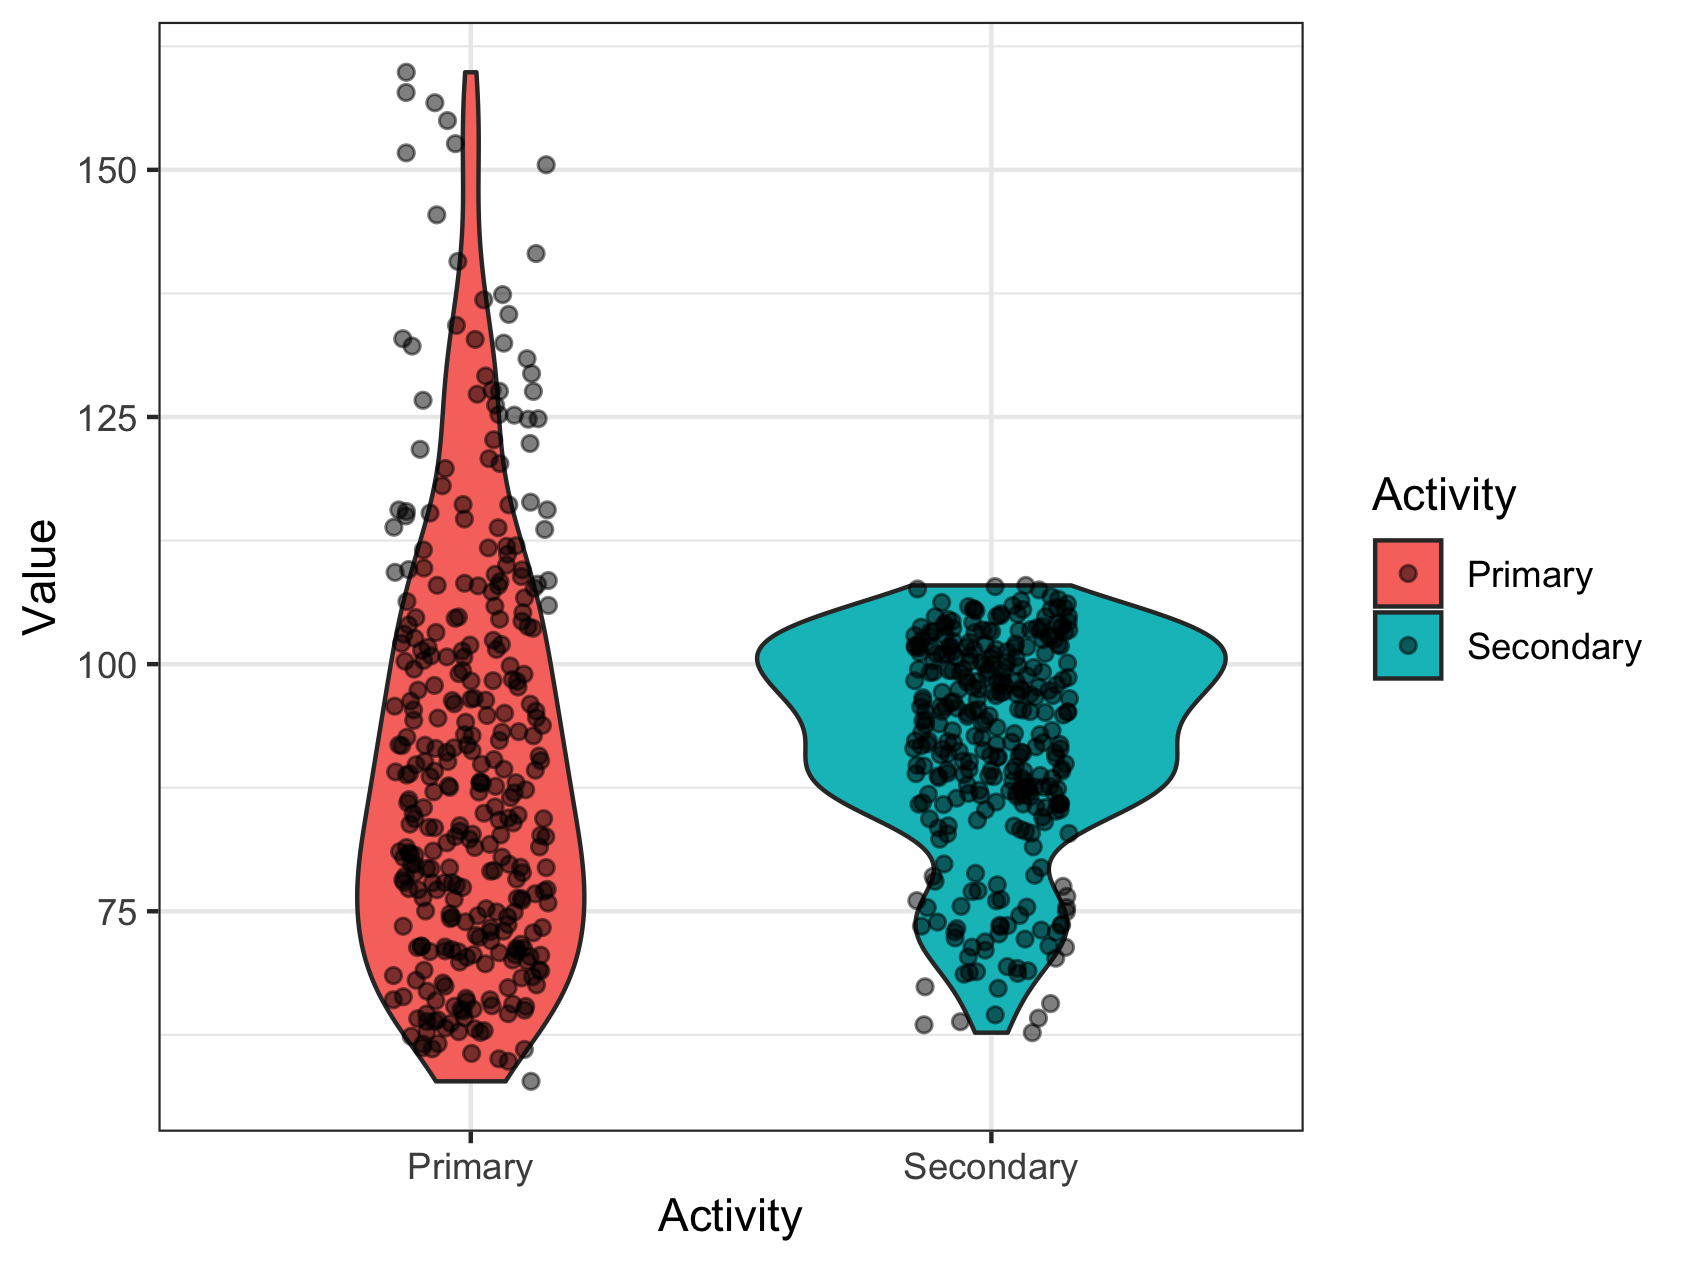
\includegraphics[scale=0.17]{extras/violin}
				\captionof{figure}{Violinplot of Primary and Secondary Activities}
				\label{fig:violin}
			\end{center}
		\end{figure}
		
		\subsection{Fisher's $ F $-Test}
		
		Fisher's $ F $-test can be used to check if two samples have the same variance \citep{selva2016}. For this case, data of secondary and tertiary activities are taken as samples. The $p$-value is $2.20\times 10^{-16}$, so the null hypothesis is rejected, which means the two samples do not have the same variance. 
		
		\VerbatimInput{extras/fisher.txt}
		
		\subsection{Chi-Squared Test}
		
		It can be used to test if two categorical variables are dependent, by means of a contingency table \citep{selva2016}. In this case, the experiment is performed to evaluate if the results of the level of activities that conform to the IGAE is independent to the months in the year 1993.
		
		For this test, there are two ways to tell if the variables are independent. The first one if by looking at the $p$-value, which in this case is 0.9931, as is greater than 0.05, the null hypothesis that the two variables are independent can not be rejected. Also, if look at the calculated Chi-Squared value, it is 9.0381, which is less than 33.9244 (critical value), so it also indicates the null hypothesis can not be rejected. In conclusion, as the two approaches lead to the same conclusion, it can be said there is no evidence to reject that the two variables are independent.  
		

		\VerbatimInput{extras/chi_squared.txt}
		
		\subsection{Correlation}
		
		Correlation is used to test the linear relationship of two continuous variables. In this case, data come from primary and secondary activities. The $p$-value is $2.20\times 10^{-16}$, which indicates the null hypothesis that there is a true correlation between the two variables is rejected. Figure \ref{fig:correlation} a scatter plot is generated in order to show how data is distributed. 
		
		\VerbatimInput{extras/correlation.txt}
		
		\begin{figure}
			\begin{center}
				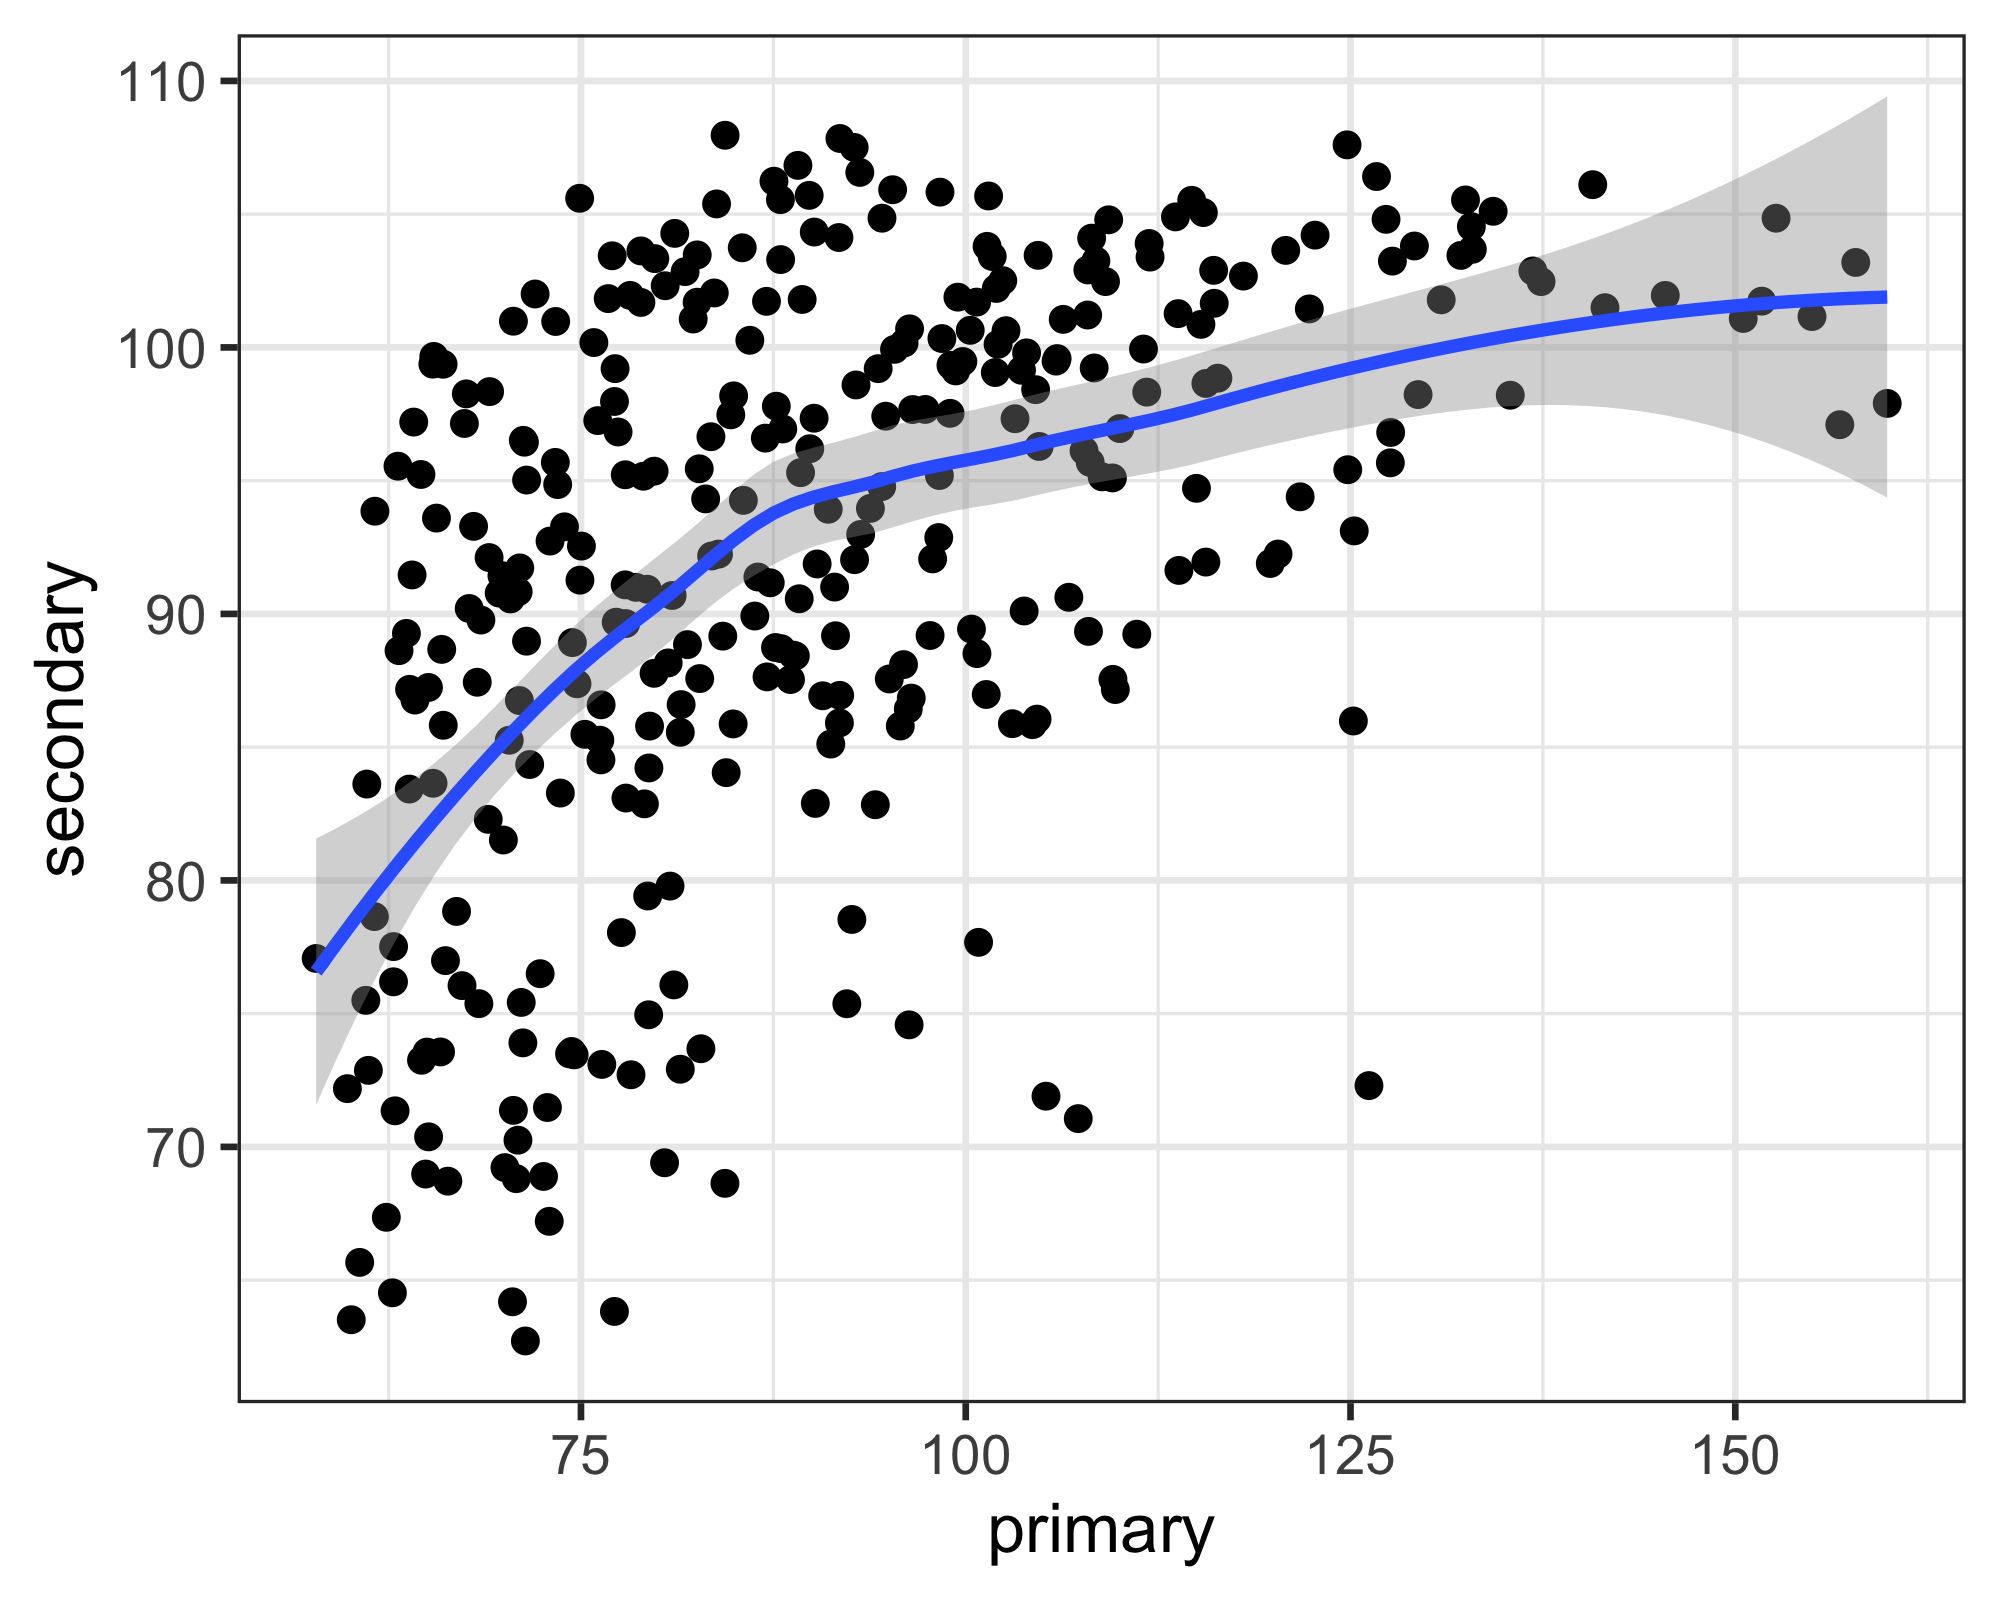
\includegraphics[scale=0.15]{extras/scatter}
				\captionof{figure}{Scatterplot of Primary and Secondary Activities}
				\label{fig:correlation}
			\end{center}
		\end{figure}
		
		
		
\clearpage

	\bibliography{tarea6}
	\bibliographystyle{plainnat}
	
\end{document}